\documentclass[a4paper,12pt,titlepage,final]{book}

\usepackage[utf8]{inputenc} \usepackage[spanish]{babel}
\usepackage{graphicx}
\usepackage{listings}
\usepackage{color}
\usepackage{amsmath}
\usepackage[round,sort,comma]{natbib}
\usepackage[titletoc]{appendix}

\definecolor{dkgreen}{rgb}{0,0.39063,0}
\definecolor{dkgrey}{rgb}{0.2,0.2,0.2}
\definecolor{grey}{rgb}{0.99,0.99,0.99}
\definecolor{DarkOrchid}{rgb}{0.80,0.0,0.80}

\renewcommand{\appendixname}{Apéndices}
\renewcommand{\appendixtocname}{Apéndices}
\renewcommand{\appendixpagename}{Apéndices}

\renewcommand{\lstlistingname}{Listado}
\lstset{
language=Verilog,
frame=shadowbox,
numbers=left,
captionpos=b,
basicstyle=\footnotesize,
backgroundcolor=\color{grey},
rulesepcolor=\color{dkgrey},
keywordstyle=\color{blue},
commentstyle=\color{dkgreen},
stringstyle=\color{DarkOrchid},
tabsize=3,
breaklines=true,
breakautoindent=true
xleftmargin=2em,xrightmargin=2em, aboveskip=1em,
}
   
\title{\Huge ACELERACIÓN DEL ALGORITMO SOBEL MEDIANTE UNA FPGA}

\author{Rafael Waldo Delgado Doblas}

\date{Curso 2012 - 2013}

\begin{document}

\frontmatter

\begin{titlepage}
\begin{center}
\vspace*{-1in}
\begin{figure}[htb]
\begin{center}

\includegraphics[width=8cm]{./figuras/Logo_ULL.png}
\end{center}
\end{figure}
\vspace*{0.15in}
ESCUELA TÉNICA DE INGENIERÍA INFORMÁTICA\\
\vspace*{0.6in}
\begin{large}
PROYECTO FINAL DE CARRERA:\\
\end{large}
\vspace*{0.2in}
\begin{Large}
\textbf{ACELERACIÓN DEL ALGORITMO SOBEL MEDIANTE UNA FPGA} \\
\end{Large}
\vspace*{0.3in}
\begin{large}
Por Rafael Waldo Delgado Doblas\\
\end{large}
\vspace*{0.3in}
\rule{80mm}{0.1mm}\\
\vspace*{0.1in}
\begin{large}
Dirigido por: \\
Jonay Tomás Toledo Carrillo \\
\end{large}
\end{center}
\end{titlepage}

\maketitle

% Definimos una primera pagina para los agradecimientos
\newpage
\thispagestyle{empty}
\section*{}
\paragraph{}
A mis abuelos, padres y hermano. \newline
Sin ellos yo no hubiera llegado donde\newline
estoy hoy, ni llegaría a donde estaré\newline
mañana.

\tableofcontents

\mainmatter
\chapter{''Descripción del documento.''}
\section*{}
\subsection*{}
\subsubsection*{}

\paragraph{}
Este documento contiene la memoria del proyecto de fin de carrera de Rafael Waldo Delgado Doblas. Este documento está estructurado de la siguiente manera:

\begin{itemize}
  \item En el primer capítulo se habla sobre las motivaciones que han llevado a realizar el proyecto.
  \item A continuación se definirán los requisitos del proyecto.
  \item Después se detallan la metodología empleada y las herramientas utilizadas.
  \item En el siguiente apartado se expondrán los pasos seguidos en el desarrollo del proyecto.
  \item Seguidamente se explica el funcionamiento del dispositivo desarrollado.
  \item Para finalizar se presentan los resultados obtenidos.
\end{itemize}

\chapter{''Introducción.''}
\label{chap:intro}

\section{Descripción del problema.}
\subsection*{}
\subsubsection*{}

\paragraph{}
Si la primera revolución industrial se estudia en los libros como un hito en la historia de la humanidad, por los cambios sociales y de organización del trabajo que supuso. En la actualidad se esta viviendo lo que se puede considerar como otra gran revolución tecnológica, en este caso la revolución viene marcada por la informática que está dando lugar a un cambio importantísimo en todas las áreas del conocimiento humano. El desarrollo de las tecnologías de la información y la comunicación han cambiado para siempre la forma en la que interactuamos con las máquinas y la forma en la que éstas desarrollan sus funciones, así como la manera de relacionarse las personas entre si.

\paragraph{}
Esta revolución es además algo vivo y en continua evolución hablar de aquellos primeros ordenadores y compararlos con los actuales es como retroceder a una época arcaica. Los avances que para nosotros ahora son un logro importantísimo dentro de unos años solamente habrán sido un paso hacia delante en este continuo evolucionar de un área del conocimiento en permanente desarrollo. En el día a día podemos ver como surgen nuevos dispositivos, cada vez más pequeños, con más capacidad computacional, un menor consumo energético y una decidida y clara orientación a facilitar nuestro que hacer diario.

\paragraph{}
Uno de esos grandes logros en principio inalcanzable sería el de conseguir que las futuras máquinas pudieran adquirir los sentidos humanos y entre ellos el sentido de la vista fundamental para nosotros. Para los seres humanos la vista es el sentido más importante a la hora de obtener información del entorno físico que le rodea. Con ella nos movemos con precisión, siendonos necesaria para casi cualquier acción que realizamos; desde algo tan simple como seleccionar la ropa que vamos a vestir hasta inspeccionar, haciendo uso de un microscopio, como se ha desarrollado un determinado cultivo de una investigación, requieren de nuestra habilidad para ver. Por eso no es de extrañar que una de las áreas de la inteligencia artificial que más importancia y desarrollo está teniendo a día de hoy sea la visión por computador.

\paragraph{}
Se ha estudiado que el ser humano captura la luz a través de los ojos, y que esta información circula a través del nervio óptico hasta el cerebro donde se procesa. Existen razones para creer que el primer paso de este procesado consiste en encontrar elementos más simples en los que descomponer la imagen. Después el cerebro interpreta la escena y por último actúa en consecuencia.

\paragraph{}
La visión por computador es un campo que incluye métodos para adquirir, procesar, analizar y entender imágenes, por lo general obtenidas del mundo real, para producir información numérica o simbólica computable por un ordenador. La visión por computador se utiliza a día de hoy en múltiples aplicaciones; algunos ejemplos podrían ser:

\begin{itemize}
  \item Inspección automatizada en procesos industriales como por ejemplo: comprobación del llenado de ampollas, comprobación de circuitos impresos
  \item Sistemas de guiado en sistemas autónomos inteligentes.
  \item Realidad aumentada.
  \item Control por gestos en interfaces hombre máquina.
  \item Extracción de información en imágenes complejas como por ejemplo: El análisis de imágenes médicas, aéreas o submarinas.
  \item Vídeo vigilancia.
\end{itemize}

\paragraph{}
Los componentes de un sistema de visión por computador dependen mucho del tipo de aplicación. Algunos sistemas pueden ser independientes y orientados a resolver algunos problemas de detección o de medición, mientras que otros pueden constituir un subsistema de un sistema mayor que a su vez puede tener otros subsistemas como por ejemplo actuadores mecánicos, bases de datos, interfaces hombre máquina, etc. Como podemos ver muchas de las funciones del sistema serán únicos según que aplicación. Sin embargo, existen algunas funciones típicas que pueden ser encontradas en la mayoría de los sistemas de visión por computador. Estas funciones son:

\begin{itemize}
  
  \item  \textbf{Adquisición de Imágenes:} Una imagen digital puede estar producida por uno o más sensores de imagen, los cuales pueden ser de varios tipos tales como: cámaras sensibles a diferentes tipos de luz, radars, rangefinders, aparatos de tomografía, cámaras de ultrasonidos, etc. Dependiendo del tipo de sensor, la imagen resultante podrá ser en 2D, 3D o una secuencia de imágenes. La imagen estará formada por pixels que podrán representar la intensidad de luz en ese punto o otras medidas tales como la profundidad la absorción de sonido o ondas electromagnéticas.
  
  \item \textbf{Preprocesado:} Normalmente antes de que se pueda aplicar un algoritmo de visión por computador a una imagen para extraer información de esta, suele ser necesario procesar los datos de la imagen para asegurar que satisface los requisitos previos impuestos por el algoritmo. Algunos ejemplos de preprocesado son:
  \begin{itemize}
    \item Escalado de la imagen.
    \item Reducción de ruido.
    \item Aumento del contraste.
  \end{itemize}  
  
  \item \textbf{Extracción de características:} Se extraen características de la imagen a varios niveles de complejidad. Algunos ejemplos son:
  \begin{itemize}
    \item Detección de bordes.
    \item Localización de puntos de interés.
  \end{itemize}
  
  Otras características más complejas estarían relacionadas con la textura la forma o el movimiento.
  
  \item \textbf{Detección/Segmentación:} Normalmente en algún momento del procesado se deciden qué áreas de la imagen son interesantes para ser procesadas en profundidad. Un ejemplo sería:
  
  \begin{itemize}
    \item Selección de un subconjunto de puntos de interés.
    \item Segmentación de una o varias regiones de la imagen que contienen objetos de interés.
  \end{itemize}
  
  \item \textbf{Procesado de alto nivel:} En este paso la entrada suele ser normalmente un conjunto pequeño de datos, por ejemplo un conjunto de puntos o una región que debería contener un objeto específico. Aquí se realiza el resto de los trabajos de la etapa de procesado, tales como:
  
  \begin{itemize}
    \item Comprobar si los datos verifican el modelo especificado por la aplicación.
    \item Estimación de parámetros.
    \item Clasificación de un objeto detectado.
    \item Comparar y combinar diferentes vistas del mismo objeto.
  \end{itemize}
  
  \textbf{Toma de decisiones:} En este paso se realizan las decisiones finales requeridas por la aplicación. Por ejemplo:
  
  \begin{itemize}
    \item Pasar o Invalidar en inspecciones automáticas
    \item Encontrado o no Encontrado en aplicaciones de reconocimiento.
  \end{itemize}
  
\end{itemize}

\paragraph{}
Si bien en la adquisición de información visual se ha conseguido superar con creces las capacidades humanas, existiendo cámaras que pueden captar hasta quinientas mil imágenes por segundo con resoluciones que van más allá de lo percibible por el ojo humano; en el procesado de estas imágenes es donde todavía las capacidades de visión de los computadores distan mucho de las capacidades humanas.

\paragraph{}
Varios son los problemas que influyen en que las capacidades de los sistemas de visión por computador:

\begin{itemize}
  \item Necesidad de computo elevada: Los algoritmos de visión por ordenador requieren de sistemas potentes para ser ejecutados.
  \item No abundancia de hardware específico: En la actualidad la mayoría de los ordenadores no disponen de un hardware específico para realizar funciones de visión por ordenador.
  \item Limitaciones del sistema: En ocasiones las propiedades físicas, el método de refrigeración del sistema o el propio sistema, puede suponer un problema para la aplicación a implementar. Ej: Quadcopter.
  \item Alto consumo energético: El consumo energético influye tanto en el costo como en la viabilidad de implementar una aplicación en la que la energía está limitada. Ej: Un sistema autónomo inteligente cuya energía está limitada a la proporcionada por sus baterías.
  \item Alto costo: Todos los anteriores problemas descritos influyen negativamente en el costo generando sistemas caros
\end{itemize}

\paragraph{}
En este proyecto se comparan las ventajas de tener un hardware dedicado a la visión por computador frente al uso de un hardware de propósito general. Al mismo tiempo se ha buscado una sistema que permita dar solución a todos los problemas anteriores.

\section{Soluciones.}
\label{sec:soluciones}
\subsection*{}
\subsubsection*{}

\paragraph{}
Este proyecto se ha desarrollado para comprobar cómo afectaría a la eficiencia de un sistema de visión por computador, si sus algoritmos en vez de ser implementados por software fuesen implementados por hardware. Para tal efecto se ha construido un sistema básico de visión por computador y se han efectuado una serie de pruebas de rendimiento.

\paragraph{}
El sistema construido cuenta con una CPU \textit{NIOS II} desarrollada por Altera para sus FPGAs. El \textit{NIOS II} es una CPU orientada a sistemas embebidos de 32bits y tiene la ventaja de que su juego de instrucciones puede ser ampliado fácilmente. Por otra parte el sistema cuenta con una entrada de vídeo compuesto para obtener las imágenes a procesar y un LCD para mostrar los resultados.

\paragraph{}
Aprovechando la facilidad de esta CPU para ampliar su juego de instrucciones, se ha añadido una implementación hardware del algoritmo Sobel a su juego de instrucciones. Este algoritmo se ha usado para hacer las pruebas de rendimiento comparándolo con una versión escrita en C compilada para la misma CPU.

\paragraph{}
Como se puede ver en los resultados de las pruebas realizadas, anotados en este mismo documento, la implementación hardware permite procesar mucho mas rápido las imágenes para la misma frecuencia de reloj.

\chapter{''Definición de requisitos.''} 
\label{chap:defreq}

\paragraph{}
En el Capítulo~\ref{chap:intro} se han visto los problemas que presentan los sistema de visión por ordenador y una lista de posibles soluciones. En este capítulo se definen una serie de requisitos a alcanzar en este proyecto. Sin embargo no se especifica la forma concreta de implementarlos, esto sera tarea de los siguientes capítulos de este documento.

\paragraph{}
Como se vio en la Sección~\ref{sec:soluciones}, este proyecto implementará un sistema de visión por ordenador basado en Sobel para comparar la eficiencia de una implementación en FPGA contra una implementación en software. En las secciones siguientes se verán los requisitos necesarios para alcanzar ese objetivo.

\section{Requisitos del Hardware}
\paragraph{}
Estos requisitos hacen referencia a los requisitos que tiene que satisfacer la implementación del sistema de visión desde el punto de vista del hardware. 
 
\subsection{Subsistema Principal}
\paragraph{}
El primer requisito hardware es desarrollar un subsistema que incluya un procesador \textit{NIOS II}, un controlador de la memoria, un temporizador para realizar mediciones en tiempo de ejecución y los buses para comunicarse con una interfaz de usuario, un LCD, una entrada de vídeo y el subsistema de vídeo.

\subsection{Subsistema de Vídeo}
\paragraph{}
Otro de los requisito hardware es desarrollar un subsistema de vídeo que se encargue de adaptar la señal de vídeo proveniente de la entrada de vídeo a un formato que pueda ser manipulado fácilmente y mostrado por el LCD.

\subsection{Ampliación del Juego de Instrucciones}
\paragraph{}
El último de los requisitos hardware es ampliar el juego de instrucciones del procesador \textit{NIOS II}, con instrucciones que permitan calcular el Sobel sobre un frame que provenga del subsistema de vídeo.

\section{Requisitos del Software}
\paragraph{}
Estos requisitos hacen referencia a los requisitos que tiene que satisfacer el sistema de vídeo desde el punto de vista del software que lo controla.

\subsubsection{Implementar el Sobel por software}
\paragraph{}
Para satisfacer este requisito se ha de implementar, por software, los mismos algoritmos utilizados para ampliar el juego de instrucciones del procesador \textit{NIOS II}.

\subsubsection{Implementar el Firmware del Sistema.}
\paragraph{}
El firmware es el software responsable de controlar las funciones del sistema. Para satisfacer este requisito el firmware tendrá que:
\begin{itemize}
\item Inicializar los diferentes circuitos integrados usados en el sistema de vídeo.
\item Controlar e indicar que opciones han sido activadas mediante la interfaz de usuario. Esta interfaz de usuario tiene que permitir hacer lo siguiente: 
\begin{itemize}
\item Mostrar el tiempo que necesita un frame para ser procesado.
\item Activar o desactivar el procesamiento del Sobel sobre una imagen.
\item Congelar la imagen.
\item Seleccionar entre procesamiento por hardware o por software del Sobel.
\end{itemize}
\end{itemize}

\section{Requisitos de la Documentación}
\paragraph{}
Estos requisitos hacen referencia a la parte escrita del proyecto.

\subsubsection{Experimentos}
\paragraph{}
Mediante el uso de las funciones congelar y mostrar el tiempo, se tendrá que realizar una comparativa entre el tiempo requerido para procesar un frame por software y el tiempo requerido para procesar un frame por hardware. Esta comparativa se ha de incluir en la memoria.

\subsubsection{Memoria y Presentación del Proyecto}
\paragraph{}
Para dejar constancia de las acciones realizadas se ha desarrollado una memoria del proyecto, que contiene toda la información del mismo. También se ha desarrollado una presentación del proyecto para ser expuesto ante el tribunal de evaluación.

\chapter{''Herramientas y Metodología.''}

\section{Herramientas.}
\subsection{Elementos Hardware}
\subsubsection*{}

\paragraph{}
Como ya se comentó en el Capítulo~\ref{chap:defreq} este proyecto se construirá a partir del procesador \textit{NIOS II} proporcionado por Altera. Por ello se ha elegido como piedra angular el \textit{NIOS II Embedded Evaluation Kit, Cyclone III Edition} también abreviado \textit{NEEK}. 

\paragraph{}
El \textit{NEEK} se compone de una placa principal que contiene la FPGA y otros elementos básicos y una \textit{daughter board} que contiene diversos circuitos integrados de apoyo junto con un LCD. Como se puede ver este kit es idóneo para satisfacer los requisitos hardware. 

\paragraph{}
Entre los elementos que alberga la placa principal los destacables para este
proyecto serían:

\begin{itemize}
\item Una FPGA \textit{Cyclone III EP3C25F324}. Esta FPGA tiene aproximadamente unos 25000 elementos lógicos, 0.6Mb repartidos en 66 elementos de memoria de 9k, 16 multiplicadores de 18x18 bits, 4 PLLs y 214 I/Os.

\item Un \textit{USB-Blaster II} embebido en la placa para descargar la configuración de la FPGA desde el PC.

\item Un chip de memoria DDR SDRAM de 32MB con un bus de 16 bits.

\item 4 switches y 4 LEDs. Por restricciones de la FPGA solo se puede usar uno de los LEDs cuando se usa la memoria RAM.
\end{itemize}

\paragraph{}
Por otra parte la \textit{daughter board} proporciona varios tipos de entradas y salidas, aunque para este proyecto la única interesante es la entrada de vídeo compuesto. El vídeo procedente de esta entrada es decodificado por un \textit{ADV7180}, que soporta entre otros formatos \textit{PAL, PAL60 y NTSC}. Este decodificador convierte  la señal analógica al formato \textit{ITU-R BT.656 digital} con una precisión de 10 bits.

\paragraph{}
El LCD está fabricado por Toppoly cuyo modelo es \textit{TD043MTEA1}. Tiene un tamaño de 4.3”, una resolución de 800x480 y proporciona una interfaz \textit{SPI 3-Wire} para configurar los distintos registros que controlan el LCD.

\subsection{Elementos Software}
\subsubsection*{}

\paragraph{}
Por otra parte se ha empleado la suite de desarrollo proporcionada por Altera, \textit{Quartus II}. Esta suite proporciona distintas herramientas para facilitar las diferentes etapas que intervienen a la hora de desarrollar con FPGAs. Las herramientas usadas en este proyecto fueron:

\begin{itemize}
\item \textbf{QSys:} Esta herramienta genera de forma automática la lógica de interconexión entre los distintos módulos del sistema.

\item \textbf{ModelSim Altera Edition:} Esta herramienta permite simular el comportamiento de un módulo, permitiendo ver el estado de los diferentes elementos del módulo en los diferentes períodos.

\item \textbf{SignalTap:} Esta herramienta es un analizador lógico que permite analizar el estado del los diversos elementos del sistema en tiempo de ejecución.

\item \textbf{Programmer:} Permite descargar un archivo de configuración ya compilado a la FPGA.

\item \textbf{PinPlanner:} Permite asociar los pines de la FPGA a las entradas/salidas del sistema.
\end{itemize}

\subsection{Otras herramientas Altera }

\paragraph{}
Una de las ventajas de haber desarrollado el sistema con soluciones Altera, es el gran número de herramientas que Altera proporciona para facilitar la construcción de sistemas a medida. Entre las herramientas que proporciona se encuentra una gran base \textit{IPs}. Una \textit{IP} es un módulo que realiza una función determinada.

\subsubsection{IPs de Altera Utilizadas}

\paragraph{CPU NIOS II/f:}
Es la version mas rápida de la CPU \textit{NIOS II} entre cuyas características las mas destacables son:

\begin{itemize}
\item Tiene una cache para instrucciones y otra para datos.

\item Pipeline de seis estados.

\item Multiplicación en un solo ciclo.

\item Predicción de saltos.

\item Permite añadir hasta 256 instrucciones personalizadas al juego de instrucciones original.
\end{itemize}

\paragraph{}
Por otra parte Altera también proporciona un IDE para desarrollar aplicaciones en C para el \textit{NIOS II}. El IDE esta basado en Eclipse e integra varias herramientas que permiten realizar la mayoría de las acciones típicas del desarrollo de software.

\paragraph{NIOS II Floating-Point Custom Instructions:}
Añade soporte al \textit{NIOS II} para realizar operaciones en coma flotante.

\paragraph{DDR SDRAM Controller:}
Permite conectar un módulo de memoria DDR a un bus \textit{Avalon MM}.

\paragraph{Altera Video IP:}
Es una suite de \textit{IPs} que permiten realizar diversas tareas para el procesado digital de un flujo de vídeo.

\subsubsection{Buses de conexión}

\paragraph{}
Para facilitar todavía más el uso de los diferentes módulos Altera proporciona una serie de buses que permiten la interconexión entre las diferentes \textit{IPs}.

\paragraph{Avalon-MM:}
Permite el mapeo de varios elementos sobre un espacio de memoria. Este espacio es de lectura y escritura, donde pueden coexistir varios elementos maestros que accedan a varios elementos esclavos. Para evitar posibles problemas derivados por el acceso concurrente de dos o más elementos maestros a un mismo elemento esclavo, el bus proporciona un sistema de planificación \textit{Round-Robin}.

\paragraph{}
Los buses \textit{Avalon MM} permiten un modo de acceso llamado modo ráfaga. En este modo el maestro enviará/recibirá al/del esclavo un dato proveniente de un conjunto de direcciones contiguas, durante un número determinado de ciclos. La forma mas fácil de garantizar que el maestro dispondrá de los datos necesarios para realizar la ráfaga es acumulándolos en un FIFO y comenzar el envío cuando el nivel de éste haya alcanzado un tamaño igual al de la ráfaga. Por otra parte como se vio anteriormente los buses \textit{Avalon MM} presentan un sistema de planificación \textit{Round Robin}, esto nos garantiza que mientras que un maestro este accediendo al bus en el modo ráfaga, ningún otro maestro podrá interrumpirlo por lo que la transferencia se hará más rápido cuanto mayor sea el tamaño de la ráfaga, a costa de sacrificar velocidad de otros maestros. 

\paragraph{Avalon-ST:}
Este bus permite el envío de flujos de información de forma unidireccional entre dos elementos. Al ser un flujo unidireccional y solo entre dos elementos, la comunicación se simplifica mucho, reduciéndose el protocolo de handshake a una señal proveniente del emisor para indicar el deseo de iniciar la comunicación y otra señal proveniente del receptor para responder que la comunicación puede ser iniciada.

\paragraph{}
Este tipo de bus permite el envío de información empaquetada. Esta cualidad es utilizada en la suite \textit{Altera Video IP}, concretamente en los flujos de vídeo utilizados en la comunicación de las diferentes \textit{IPs}. En esta suite cada frame es enviado en dos paquetes, un primer paquete que proporciona la resolución del frame y si este se encuentra en modo entrelazado o progresivo; y un segundo paquete que contiene la información del color de cada uno de los píxeles que componen dicho frame. 

\paragraph{Custom Instruction:}
Una de las capacidades más interesantes del procesador \textit{NIOS II} es su capacidad para añadir instrucciones propias, lo que permite que pueda ser adaptado a un sin fin de situaciones. Para tal efecto Altera proporciona en su CPU el bus \textit{Custom Instruction}. Dicho bus permite el paso de operadores a la lógica de la instrucción, el acceso a los registros internos de la CPU y al bus de opcode de las instrucciones personalizadas.  

\paragraph{Avalon Interrupt:}
Este tipo de bus permite el envío de una señal de interrupción al \textit{NIOS II}.
 
\paragraph{Avalon Conduit:}
Este bus permite agrupar un conjunto de señales arbitrarias, a las cuales el usuario puede dar el rol que más le convenga. Este bus se usa para interconectar \textit{IPs} que cuyas necesidades no queden satisfechas con los anteriores buses o conectar \textit{IPs} con el mundo exterior a la FPGA.

\section{Metodología.}
\subsection{Consideraciones}
\subsubsection*{}

\paragraph{}
Al tratarse de un proyecto hardware se presentaran diversas peculiaridades propias de este tipo de proyectos. Una de las más destacadas sin duda será el hecho de que la mayor parte de las operaciones se realizarán en paralelo necesitándose por tanto diversos métodos de sincronización. Se utilizarán señales de reloj y flags para sincronizar la ejecución de los diferentes módulos.

\paragraph{}
Otra particularidad será tener en cuenta los tiempos que tarda cada módulo en terminar, porque es posible que un trigger que inicia un módulo, se dispare antes de que este modulo haya finalizado la anterior tarea.

\paragraph{}
También es importante establecer métodos para controlar el acceso concurrente a diferentes medios. Esto se realiza gracias a las interfaces Avalon comentadas anteriormente que disponen de señales para indicar si un determinado elemento esta en uso o no. Por otra parte como Verilog no permite la asignación desde diferentes módulos a un registro y estas se producen al final de la ejecución del módulo, la concurrencia entre módulos es prácticamente nula.

\paragraph{}
Por otra parte también se presentan problemas de tipo electrónico tales como: frecuencia máxima, capacitancias e inductancias entre pistas, corriente máxima que puede dar una fuente, etc. Afortunadamente el \textit{NEEK} es un hardware que ya ha sido diseñado teniendo en cuenta estos problemas con lo que a la hora de trabajar con él, lo único que habrá que tener en cuenta será el de no contrariar ninguna de las especificaciones de uso.

\subsection{Pasos para el desarrollo}
\subsubsection*{}
\paragraph{}
Para comenzar el desarrollo con el \textit{NEEK} lo primero que hay que hacer es crear un nuevo proyecto en \textit{Quartus 2}, definirle el tipo de FPGA y el archivo que servirá de modulo cabecera. Este modulo sera el que conecte sus entradas y salidas con los pines de la FPGA.

\paragraph{}
Una vez definido el proyecto dependiendo de la amplitud del mismo se pueden realizar varias técnicas, como trabajar directamente con un lenguaje HDL o arrastrando módulos de forma gráfica; sin embargo el camino normal para un proyecto de mediana o gran envergadura será utilizar \textit{QSys} como herramienta para construir el sistema.

\paragraph{}
\textit{QSys} permite de una forma gráfica acceder a una extensa librería de \textit{IPs} proporcionada por Altera e incrementar dicha librería con \textit{IPs} realzados por nosotros mismos. Estos módulos deben utilizar como entrada y salida los buses comentados con anterioridad.

\paragraph{}
Una vez construido y generado el sistema, hay que agregarlo al proyecto, instanciarlo desde el modulo cabecera y conectar las entradas y salidas del modulo cabecera a las entradas y salidas del sistema generado por \textit{QSys}.

\paragraph{}
A continuación hay que definir la asignación de los pines de la FPGA sobre el módulo cabecera, esto se realiza con el \textit{PinPlanner}.

\paragraph{}
Para terminar se genera el sistema y se programa sobre la FPGA.

\paragraph{}
Estos pasos describen la construcción de un sistema ideal que no tiene ningún fallo, sin embargo a la hora de la verdad es conveniente saber que Altera proporciona dos herramientas muy útiles para la depuración de errores. 

\paragraph{}
La primera es el \textit{ModelSim Altera Edition} que permite simular de forma independiente las \textit{IPs} desarrollados sin necesidad de generar el sistema.

\paragraph{}
Por otra parte también disponemos del \textit{SignalTap} un analizador lógico que puede ser añadido una vez el sistema haya sido generado. Para ello tenemos que definir las señales que queremos analizar y la señal de reloj que utilizan y luego volver a generar el sistema con el analizador lógico integrado. Esto tiene el problema de que el analizador lógico consume tanto elementos lógicos como elementos de memoria y es necesaria dos compilaciones con el tiempo que ello conlleva.

\paragraph{}
Como ya se comento antes para sistemas que utilicen el \textit{NIOS II} Altera proporciona un IDE para desarrollar aplicaciones en C/C++. Para comenzar a desarrollar aplicaciones lo primero sera buscar el \textit{BSP} de nuestro sistema generado por \textit{QSys}. Este archivo proporciona una descripción del sistema construido necesaria para generar el sistema operativo \textit{HAL}. \textit{HAL} es un SO que proporciona el conjunto de librerías básico de C/C++. además de algunos drivers para manejar las \textit{IPs} que así lo requieran. Una vez seleccionado el \textit{BSP} ya podemos empezar a desarrollar aplicaciones en C como si de cualquier otra plataforma se tratase.

\chapter{''Los Subsistemas.''}
\subsection*{}
\subsubsection*{}

\paragraph{}
En este capítulo se hablara de como se han implementado los subsistemas de los se compone el sistema a implementar, concretamente: el principal y el de vídeo. 

\section{Subsistema Principal}
\subsection*{}
\subsubsection*{}

\paragraph{}
En las Figuras~\ref{fig:Subsistema Principal 1-3},~\ref{fig:Subsistema Principal 2-3}~y~\ref{fig:Subsistema Principal 3-3} se puede observar como esta compuesto el subsistema principal.

\begin{figure}[p]
\centering
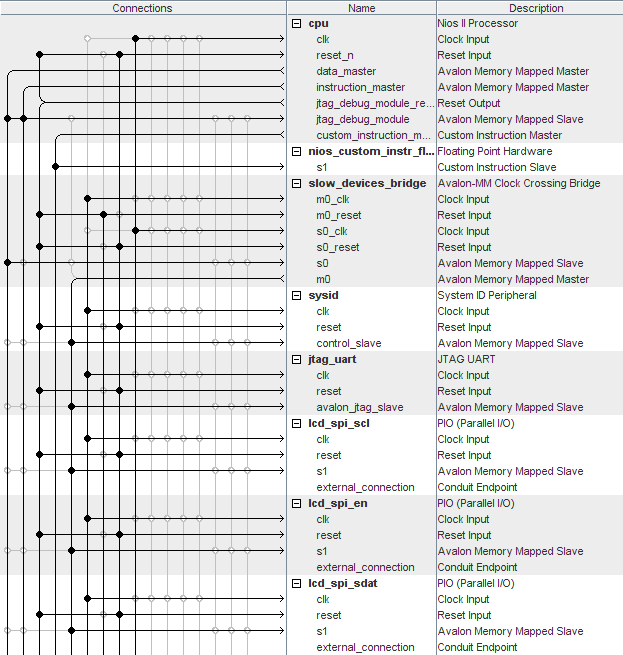
\includegraphics[height=0.95\textheight,
width=0.95\textwidth]{./figuras/SistemaPrincipal/sistemaprincipalpagina1.png}
\caption{Subsistema Principal 1-3}
\label{fig:Subsistema Principal 1-3}
\end{figure}

\begin{figure}[p]
\centering
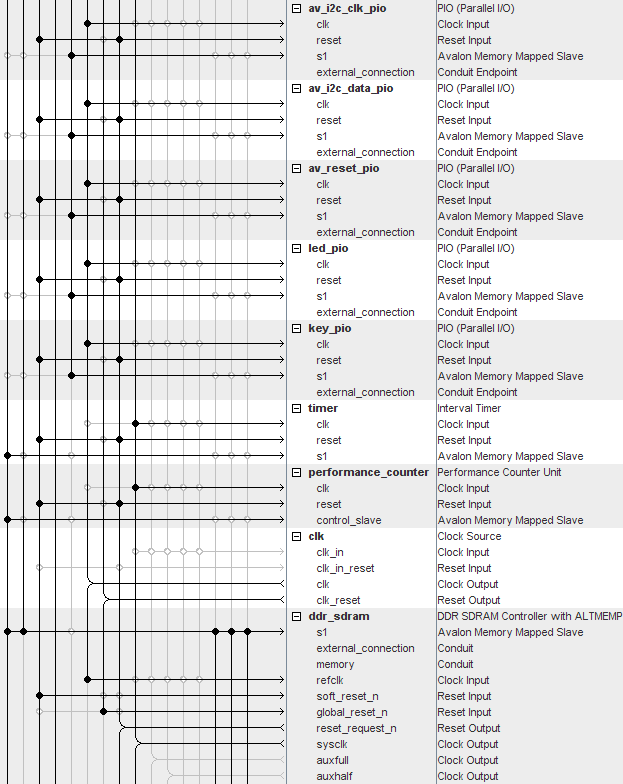
\includegraphics[height=0.95\textheight,
width=0.95\textwidth]{./figuras/SistemaPrincipal/sistemaprincipalpagina2.png}
\caption{Subsistema Principal 2-3}
\label{fig:Subsistema Principal 2-3}
\end{figure}

\begin{figure}[p]
\centering
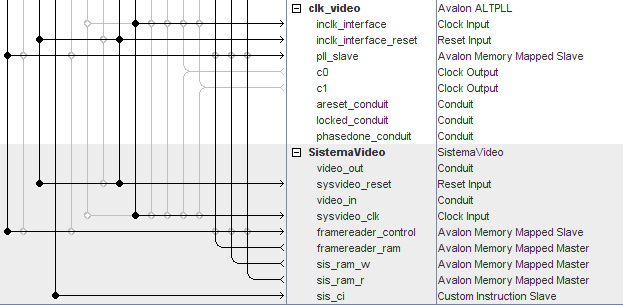
\includegraphics[height=0.5\textheight,
width=0.95\textwidth]{./figuras/SistemaPrincipal/sistemaprincipalpagina3.png}
\caption{Subsistema Principal 3-3}
\label{fig:Subsistema Principal 3-3}
\end{figure}

\paragraph{}
Como se puede apreciar los buses de datos y de instrucciones de la CPU están conectados a un bridge que adapta la velocidad de reloj de los dispositivos más lentos a la del bus del sistema. A su vez tenemos conectado al bus del sistema: la memoria RAM, diversos periféricos que permiten medir el tiempo y el subsistema de vídeo.

\paragraph{}
También hay un \textit{PLL} para generar la señal de reloj del flujo de salida de vídeo que va al LCD.

\paragraph{}
Como se puede observar se ha definido una conexión de tipo \textit{SPI 3-Wire}. Esta conexión permite configurar el LCD, para ello hay un conjunto de librerías que facilitan la tarea de configurarlo desde C. 

\paragraph{}
Por otra parte se tiene otra conexión tipo \textit{I2C}. Esta conexión permite configurar el  decodificador de vídeo. También tenemos dos buses de 4 bits para el control de los LED y de los pulsadores.

\paragraph{}
El sistema de vídeo tiene acceso directo al bus del sistema permitiéndole leer y escribir directamente sobre la memoria RAM.

\section{Subsistema de Vídeo}
\subsection*{}
\subsubsection*{}

\paragraph{}
Por otra parte en la Figura~\ref{fig:Sistema Video} se puede apreciar como está construido el subsistema de vídeo.
\begin{figure}[p]
\centering
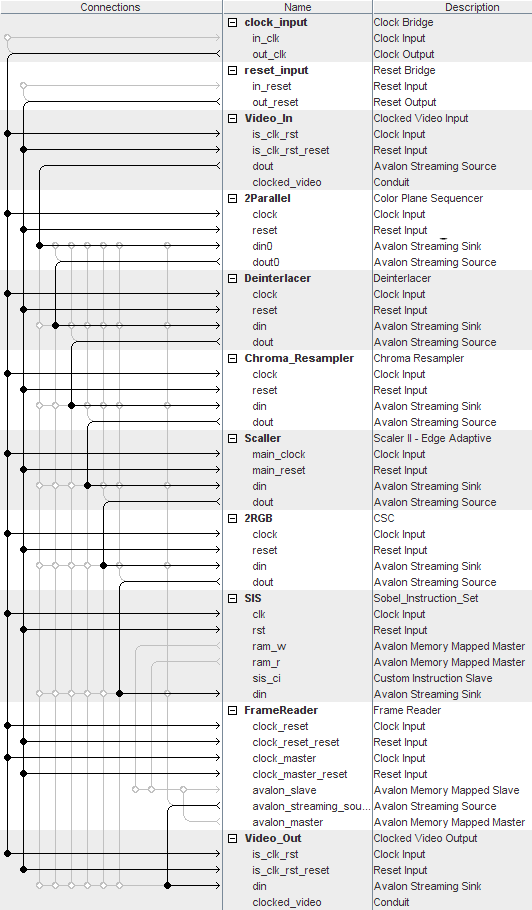
\includegraphics[height=0.95\textheight,
width=0.95\textwidth]{./figuras/SistemadeVideo/sistemadevideopagina1.png}
\caption{Subsistema Vídeo}
\label{fig:Sistema Video}
\end{figure}

\paragraph{}
Este sistema realiza varias acciones que se analizaran en las siguientes secciones.

\subsection{Obtención del flujo de vídeo}
\subsubsection*{}

\paragraph{}
La primera es transformar un flujo de vídeo en formato \textit{ITU-R BT.656} a el formato \textit{RGB 4:4:4}. Se eligió trabajar en este formato por ser el más fácil de manipular a la hora de trabajar. Para realizar esta acción se han utilizado varios módulos de Altera:

\paragraph{}
El primero es el \textit{Clocked Video Input}: Este modulo se encarga de convertir las señales provenientes del decodificador de vídeo a un flujo Vídeo Avalon.

\paragraph{}
Una vez que tenemos un flujo de vídeo Avalon podemos utilizar el resto de IPs de la suite \textit{Altera Video IP}.

\paragraph{}
La siguiente IP que nos encontramos es el \textit{Color Plane Sequencer}, este módulo hace que los planos \textit{Y} y \textit{C} del flujo pasen de estar en secuencia a estar en paralelo. Esto facilita el manejo de la información porque se puede disponer de toda la información de un píxel de forma simultanea.

\paragraph{}
Después utilizamos un \textit{Deinterlacer} para desentrelazar la señal de vídeo. Esto es importante porque el Sobel trabaja mirando los píxeles de las líneas inferior y superior.

\paragraph{}
A continuación utilizamos la IP \textit{Chroma Resampler} para convertir el flujo de muestreo con formato \textit{4:2:2} a formato \textit{4:4:4}, con esto conseguimos que todas las componentes tengan la misma longitud en bits por lo que facilita su manejo.

\paragraph{}
Seguidamente escalamos los frames con un \textit{Scaller} para que sus dimensiones coincidan con las del LCD.

\paragraph{}
Para finalizar con el modulo \textit{CSC} se cambia el espacio de color YCbCr a RGB, que como ya hemos dicho resulta mas fácil de manejar.

\paragraph{}
De esta forma hemos conseguido un flujo de video RGB Avalon en paralelo de 24 bits de ancho con 8 bits por canal de color cuyos frames tienen las dimensiones adecuadas para ser adecuadas para ser mostrados en un LCD. Este flujo es inyectado en la IP \textit{Sobel Instuction Set} para ser tratado.

\subsection{Mostrar el frame}
\subsubsection*{}

\paragraph{}
Otra de las acciones que realiza este sistema es la de leer de memoria un frame y mostrarlo por pantalla. Para ello volvemos hacer uso de la suite \textit{Altera Video IP}.

\paragraph{}
La primera \textit{IP} usada en esta tarea es el \textit{FrameReader}, esta \textit{IP} lee un frame en formato RGB paralelo de 24 bits y lo transforma a un flujo de vídeo Avalon. A continuación con un \textit{Clocked Video Output} se genera el conjunto de señales necesarias para mostrar el frame en el LCD.

\subsection{Procesado de la información}
\subsubsection*{}
\paragraph{}
La última de las acciones del subsistema de vídeo consiste en aplicar varios procesados a los frames y almacenar los resultados en memoria. Esta acción sera el núcleo de este proyecto, donde se ha usado una \textit{IP} desarrollada por mi, \textit{Sobel Instruction Set}, que contiene las instrucciones necesarias para aplicar el Sobel en un flujo de vídeo. Para su comunicación con el exterior, presenta cuatro buses: dos de tipo \textit{Avalon MM} para la lectura y escritura de datos en la memoria, uno de tipo \textit{Avalon ST} para la entrada del flujo de vídeo y otro de tipo \textit{Custom Instruction} para comunicar la \textit{IP} con el procesador \textit{NIOS II}. 

\paragraph{}
Al contener varias instrucciones ha sido necesario añadir una lógica de control para decodificar los distintos opcodes que vienen del procesador. Por otra parte se ha utilizado FIFOs para aumentar las tasas de escritura y lectura de los buses \textit{Avalon MM} mediante el uso del modo ráfaga; y caches para disminuir accesos innecesarios por parte de los mismos.

\paragraph{}
En el capitulo~\ref{sec:SIS} se estudiará más en profundidad las diferentes instrucciones que componen el \textit{Sobel Instruction Set}.

\chapter{''El Sobel Instruction Set.''} \label{sec:SIS}
\section*{}
\subsection*{}
\subsubsection*{}

\paragraph{}
Como ya se comentó el \textit{Sobel Instruction Set} es el alma central del proyecto. Esta compuesto por tres instrucciones, básicas para el correcto cálculo del Sobel: \textit{FrameWrite}, \textit{AGrises} y \textit{Sobel}. Estas serán estudiadas en las siguientes secciones de este capítulo. Por otra parte estas funciones hacen uso de varios módulos de apoyo que serán comentados en la secciones que corresponda. Por último En el anexo~\ref{fig:Sistema Video} se puede ver los códigos de cada uno de los módulos que conforman el \textit{Sobel Instruction Set}.

\section{FrameWriter}
\subsection*{}
\subsubsection*{}

\paragraph{}
La primera instrucción que se debe ejecutar para poder calcular el Sobel es \textit{FrameWriter}. Esta instrucción es fundamental porque es la encargada de grabar un frame completo en memoria. Para ello una vez activada queda a la escucha en bus \textit{Avalon ST}, a la espera de detectar el comienzo de un paquete de datos con la información de los píxeles de un frame. Una vez detectado el comienzo del paquete se empieza a grabar la información píxel a píxel al modulo \textit{ram\_w} que se encargara de gestionar la escritura a ráfagas de la información.

\paragraph{}
En los listados~\ref{lst:DeteccionFW}~y~\ref{lst:EscrituraFW} se puede ver en detalle el sistema de detección de comienzo de frame y la escritura respectivamente. 

\lstinputlisting[caption=Detección de Frame,label=lst:DeteccionFW,linerange={68-69},firstnumber=68]{./SISSources/V/FrameWriter.v}

\paragraph{}
Como se puede ver cuando se detecta el inicio de un paquete \textit{din\_sop}, el dato de entrada es 0 \textit{din\_data}, el ciclo es válido \textit{din\_valid} y la instrucción esta en ejecución \textit{run}; se activa el flag \textit{video\_reg}.

\paragraph{}
Por otra parte \textit{video\_reg} se desactiva cuando se detecta el fin de un paquete \textit{din\_eop}, el ciclo es válido \textit{din\_valid} y éste estaba activado.

\lstinputlisting[caption=Escritura FrameWriter,label=lst:EscrituraFW,linerange=71-74,firstnumber=71]{./SISSources/V/FrameWriter.v}

\paragraph{}
La escritura en el modulo \textit{ram\_w} se produce cuando el módulo ha sido activado, el flag \textit{video\_reg} se encuentra activo y el emisor esta enviando datos validos \textit{din\_valid}. Si el módulo \textit{ram\_w} indica que sólo queda un hueco en su FIFO, la instrucción puede ordenar al emisor que pare haciendo uso de la señal \textit{din\_ready}. 

\section{AGrises}
\subsubsection*{}
\paragraph{}
Una vez que se tiene un frame en memoria, el siguiente paso necesario sera convertirlo a grises. Para ello tenemos la función \textit{Agrises}. Esta función hace uso del ya conocido modulo \textit{ram\_w} y del modulo \textit{ram\_r} para gestionar las escrituras y lecturas en ráfaga a/desde la memoria RAM.

\paragraph{}
Esta función hace la conversión de un píxel en dos etapas. El motivo de hacerlo en dos etapas en vez de una se debe a un problema a la hora de calcular la ecuación~\ref{eq:fgrismala}.

\begin{equation}\label{eq:fgrismala}
gris = \frac{30*rojo + 59*verde + 11*azul}{100}
\end{equation}

\paragraph{}
Si tenemos en cuenta que cada componente de color es un numero de 8 bits, el resultado del dividendo será un número de 15 bits. Por lo tanto tendremos tres multiplicaciones de 8 bits, tres sumas de 14 bits y una división de 15 bits, que no se pueden realizar en el tiempo que da un solo ciclo, incluso si se hacen las 3 multiplicaciones en paralelo porque de por sí la división de 15 bits no puede ser ejecutada en un solo ciclo. 

\paragraph{}
Para evitar este problema se optó por realizar la división en dos partes, quedando la ecuación anterior como se muestra en la ecuación~\ref{eq:fgrisbuena}.

\begin{subequations}\label{eq:fgrisbuena}
\begin{align}
        g\_aux_{[14..0]}&=30*rojo + 59*verde + 11*azul\\
        gris &= \frac{g\_aux_{[14..8]}}{0.5}+\frac{g\_aux_{[14..8]}}{2}+\frac{g\_aux_{[14..8]}}{19}+\frac{g\_aux_{[7..0]}}{64}
\end{align}
\end{subequations}

\paragraph{}
Ahora todas las divisiones son de 8 bits, por lo que se pueden ejecutar más rápido y separar las que haga falta.

\paragraph{}
Para que se inicie la primera etapa tienen que darse una serie de condiciones que se pueden observar en el listado~\ref{lst:LecturaAG}.

\lstinputlisting[caption=Lectura AGrises,label=lst:LecturaAG,linerange=89-89,firstnumber=89]{./SISSources/V/AGrises.v}

\paragraph{}
Una de las condiciones es que en el FIFO de \textit{ram\_r }haya suficientes elementos para completar una ráfaga. Otra que haya espacio en el FIFO de \textit{ram\_w}. También es necesario que la función este en ejecución. Por último el registro \textit{stages} debe de estar a cero, lo que indica que no se esta procesando algún otro píxel.

\paragraph{}
En el listado~\ref{lst:EtapasAG} se puede ver el código correspondiente a las dos etapas. En la primera etapa calculamos \textit{g\_aux} y la primera y segunda fracción de gris; y en la segunda etapa terminamos de calcular gris.

\lstinputlisting[caption=Etapas AGrises,label=lst:EtapasAG,linerange=66-87,firstnumber=66]{./SISSources/V/AGrises.v}

\paragraph{}
Una vez calculado el valor de gris en la segunda etapa, éste se pasa al módulo \textit{ram\_w} que se encargará de escribirlo en la memoria RAM. Este proceso se puede observar en el listado~\ref{lst:EscrituraAG}

\lstinputlisting[caption=Etapas AGrises,label=lst:EscrituraAG,linerange=93-94,firstnumber=93]{./SISSources/V/AGrises.v}

\section{Sobel}
\subsubsection*{}
\paragraph{}
Una vez que tenemos un frame en escala de grises en memoria, podremos calcular el Sobel propiamente dicho. Para esta tarea se dispone de la función Sobel. Esta función utilizará nuevamente el módulo \textit{ram\_w} para escribir los resultados en memoria, sin embargo para las lecturas se ha optado por utilizar una memoria cache, implementada en el módulo \textit{cache\_sobel}.

\paragraph{}
El algoritmo Sobel recorre píxel a píxel el frame, analizando los píxeles adyacentes del píxel para el cual se está calculando el valor de Sobel. Esto quiere decir que el uso de la memoria cache beneficia enormemente al Sobel porque ahorra tener que estar constantemente accediendo a memoria para obtener datos de las líneas actual, superior e inferior. Por otra parte esta memoria puede ir obteniendo los datos de líneas siguientes mientras se calculan las diferentes etapas en el calculo del Sobel, este paralelismo permite reducir significativamente las latencias de lectura.

\paragraph{}
La memoria cache implementada puede almacenar hasta un total de 10 líneas de 800 píxeles, realizar una lectura y una escritura de forma simultanea; y utiliza una política de remplazo FIFO. La mejora obtenida con respecto a la version preliminar que usaba el módulo \textit{ram\_r} fue de alrededor de un cien por cien.

\paragraph{}
En la ecuación~\ref{eq:sobel} podemos ver la expresión matemática del algoritmo para calcular el gradiente Sobel.

\begin{subequations}\label{eq:sobel}
\begin{align}
\begin{bmatrix}
G_x
\end{bmatrix}=
\begin{bmatrix}
-1 & 0 & 1\\
-2 & 0 & 2\\
-1 & 0 & 1
\end{bmatrix}*
\begin{bmatrix}
g_{nw} & g_n & g_{ne}\\
g_w & g_c & g_e\\
g_{sw} & g_s & g_{se}
\end{bmatrix}\label{eq:sobelgx}\\
\begin{bmatrix}
G_y
\end{bmatrix}=
\begin{bmatrix}
-1 & -2 & -1\\
0 & 0 & 0\\
1 & 2 & 1
\end{bmatrix}*
\begin{bmatrix}
g_{nw} & g_n & g_{ne}\\
g_w & g_c & g_e\\
g_{sw} & g_s & g_{se}
\end{bmatrix}\label{eq:sobelgy}\\
G=\sqrt{G_x^2 + G_y^2}\label{eq:sobelg}
\end{align}
\end{subequations}

\paragraph{}
Como se puede observar la ecuación~\ref{eq:sobelgx} calcula la \textit{componente x} del gradiente, para ello calcula la diferencia de brillo entre los píxeles que están a la derecha, con los que están a la izquierda, ponderando el valor de los que son adyacentes el doble de los que están en las diagonales. La ecuación~\ref{eq:sobelgy} hace lo propio pero para la \textit{componente y} del gradiente que es la vertical.

\paragraph{}
La ecuación~\ref{eq:sobelg} calcula la magnitud gradiente resultante de las \textit{componentes x} e \textit{y}. Sin embargo esta presenta un problema a la hora de implementarlo en una FPGA. La raíz cuadrada consume demasiados elementos lógicos y tiempo, sin embargo según podemos leer en [p. 218] \citet{Myler} en este caso la magnitud del gradiente puede ser aproximada de forma aceptable mediante la ecuación~\ref{eq:sobelgaprox}.

\begin{equation}\label{eq:sobelgaprox}
G_{aprox}=|G_x| + |G_y|
\end{equation}

\paragraph{}
El Sobel a sido implementado en 8 etapas. Como se puede ver en el listado~\ref{lst:EtapaIaS}, la primera etapa comenzara siempre que:

\begin{itemize}
 \item No se este procesando otro píxel \textit{stage}.
 \item Queden píxeles por procesar \textit{pixel\_counter}.
 \item Haya espacio en el FIFO de \textit{ram\_w, usedw\_fifo\_out}.
 \item Se dispongan de al menos tres líneas en la cache \textit{cache\_valid\_lines}.
\end{itemize}

\lstinputlisting[caption=Etapas Sobel,label=lst:EtapaIaS,linerange=94-94,firstnumber=94]{./SISSources/V/Sobel.v}

\paragraph{}
Cuando se activa el \textit{flag go\_sobel}, se comprobará si el píxel a analizar se encuentra en la primera columna del frame. Esto se hace porque en si no esta en esa columna, se podrán reutilizar los elementos de la matriz g, desplazando los elementos de la segunda columna a la primera y de la tercera a la segunda, solo siendo necesario obtener de la cache los elementos de la tercera columna. Por otra parte si el píxel esta en la primera columna, la columna 0 de g sera inicializada con 0s por caer fuera del frame y asumirse que el valor de fuera de la imagen es 0. En el listado~\ref{lst:EtapaIbS} se puede ver el código que realiza esta acción.

\pagebreak
\lstinputlisting[caption=Etapas Sobel,label=lst:EtapaIbS,linerange=234-247,firstnumber=234]{./SISSources/V/Sobel.v}

\paragraph{}
Por otra parte cuando esté flag este activo, se configuran las dirección en cache del píxel superior izquierdo con respecto al píxel a analizar y se configurará el número de píxeles a leer. 6 en el caso de que sea la columna 0 y 3 en caso contrario.

\paragraph{}
Al mismo tiempo se iniciará la primera etapa lo que desactivará el \textit{flag go\_sobel}.

\paragraph{}
Durante la primera etapa se leerá de la cache los píxeles necesarios y se almacenarán en la casilla correspondiente de g. En caso de que el píxel esté fuera de la imagen se asignará un valor de 0 tal y como se puede observar en el listado~\ref{lst:Etapa1S}.

\lstinputlisting[caption=Etapa 1 Sobel,label=lst:Etapa1S,linerange=248-254,firstnumber=248]{./SISSources/V/Sobel.v}

\paragraph{}
En la segunda etapa se calcularán las componentes izquierda, derecha, superior e inferior. Como se puede ver en el listado~\ref{lst:Etapa2S}

\lstinputlisting[caption=Etapa 2 Sobel,label=lst:Etapa2S,linerange=255-260,firstnumber=255]{./SISSources/V/Sobel.v}

\paragraph{}
En la tercera etapa se calcularán los valores absolutos de las compentes horizontal y vertical. Como se puede ver en el listado~\ref{lst:Etapa3S}

\lstinputlisting[caption=Etapa 3 Sobel,label=lst:Etapa3S,linerange=261-264,firstnumber=261]{./SISSources/V/Sobel.v}

\paragraph{}
En la cuarta etapa se calculará la magnitud del gradiente tal y como se explicó anteriormente. Como se puede ver en el listado~\ref{lst:Etapa4S}

\lstinputlisting[caption=Etapa 4 Sobel,label=lst:Etapa4S,linerange=265-267,firstnumber=265]{./SISSources/V/Sobel.v}

\paragraph{}
Las etapas 5 y 6 hacen que el color de los bordes sea negro y el de las llanuras blanco. Por último la etapa 7 se pasa el valor resultante a \textit{ram\_w} para que lo escriba en memoria. Esto se puede observar en los listados~\ref{lst:Etapa56S}~y~\ref{lst:Etapa7S} respectivamente.

\lstinputlisting[caption=Etapas 5 y 6 Sobel,label=lst:Etapa56S,linerange=268-273,firstnumber=268]{./SISSources/V/Sobel.v}

\lstinputlisting[caption=Etapa 7 Sobel,label=lst:Etapa7S,linerange=278-279,firstnumber=278]{./SISSources/V/Sobel.v}

\chapter{''El Firmware''}
\section*{}
\subsection*{}
\subsubsection*{}

\paragraph{}
Hasta ahora se ha hablado de la implementación del sistema Sobel desde el punto de vista del hardware, sin embargo todo sistema que involucre una CPU necesita de un pequeño software que se encargue de controlar el funcionamiento del mismo. Este pequeño software es llamado Firmware y como ya se dijo en capítulos anteriores en el caso del procesador NIOS II de Altera proporciona un IDE para desarrollar aplicaciones en C. En las subsiguientes secciones de este capítulo se irá mostrando los diferentes elementos que componen el firmware.

\section{Hardware Abstraction Layer}
\paragraph{}
El \textit{Hardware Abstraction Layer} es la pieza de software mas importante del firmware. Se encarga de facilitar la tarea de desarrollar aplicaciones proporcionando una serie de drivers para controlar las diferentes \textit{IPs} mapeadas en memoria del sistema. También proporciona la librería estándar de C, funciones para el control del temporizador y funciones para la lectura y escritura a memoria.

\section{Librerías Proporcionadas por Altera}
\paragraph{}
Para facilitar el desarrollo de aplicaciones usando diferentes \textit{IPs} Altea proporciona varias librerías. En las siguientes subsecciones de esta sección se detallarán las mas interesantes.
\subsection{Alt\_TPO\_LCD}

\paragraph{}
Esta librería permite inicializar el LCD del Altera \textit{NIOS II Embedded Evaluation Kit}. La librería utiliza la conexión \textit{SPI 3-Wire} del controlador LCD para inicializar los diferentes registros del control. En el listado~\ref{lst:alttpolcd} se puede ver las funciones que presenta esta librería.

\lstinputlisting[caption=Alt\_TPO\_LCD,label=lst:alttpolcd,linerange=42-58,firstnumber=42,language=c]{./SISSources/C/alt_tpo_lcd.h}

\paragraph{}
La estructura \textit{alt\_tpo\_lcd} alberga las direcciones de memoria de las señales que conforman el bus \textit{SPI 3-wire}.

\paragraph{}
Por otra parte la función alt\_tpo\_lcd\_init inicializa el controlador LCD con la resolución que se le indique mediante los parámetros \textit{width} y \textit{height}.

\subsection{Audio\_TVDecoder}
\paragraph{}
Esta librería permite inicializar el DAC de video compuesto del Altera \textit{NIOS II Embedded Evaluation Kit}. Para ello utiliza la conexión \textit{I2C} del circuito integrado para escribir en sus diferentes registros de control. Esta librería contiene dos ficheros cabecera, El primero presentado en el listado~\ref{lst:audiotvdecoderfunciones} se puede ver las funciones relacionadas con el control propiamente dicho del decodificador de vídeo; por otra parte en el segundo que se puede observar en el listado~\ref{lst:i2cfunciones} contiene las funciones para establecer una conexión \textit{I2C}.

\lstinputlisting[caption=Audio TV Decoder,label=lst:audiotvdecoderfunciones,linerange=24-27,firstnumber=24,language=c]{./SISSources/C/tvdecoder_ctrl.h}


\lstinputlisting[caption=I2C,label=lst:i2cfunciones,linerange=31-37,firstnumber=31,language=c]{./SISSources/C/i2c.h}


\subsection{Framereader}
\paragraph{}
Esta librería no esta proporcionada como tal por Altera si no que es un subconjunto del API de la suite \textit{Altera Video IP} que contiene solamente las funciones necesarias para manejar la \textbf{IP Frame Reader}. En el listado~\ref{lst:vipfunciones} se puede observar las funciones que proporciona.

\clearpage
\lstinputlisting[caption=Frame Reader,label=lst:vipfunciones,linerange=22-30,firstnumber=22,language=c]{./SISSources/C/vip_wrapper_for_c_func.h}

\subsection{Alt\_Video\_Display, Fonts, Graphics\_Lib}
\paragraph{}
Estas librerías permiten escribir caracteres en el LCD. 

\subsubsection{Alt\_Video\_Display}
\paragraph{}
Proporciona una estructura adecuada para almacenar la información de un frame en memoria.

\subsubsection{Fonts}
\paragraph{}
Como su nombre indica proporciona un conjunto de fuentes para poder escribir.

\subsubsection{Graphics\_Lib}
\paragraph{}
Este librería es la principal encargada de proporcionar un conjunto de funciones que permita la escritura de caracteres en el LCD.

\section{Librerías Desarrolladas por Mi}
\paragraph{}
En esta sección veremos dos librerías desarrolladas que he desarrollado para la implementación del firmware.

\subsection{Keyhandler}
\paragraph{}
Como su nombre indica la librería \textit{keyhandler} se encarga de manejar las pulsaciones de los botones. Concretamente se encarga de gestionar las interrupciones generadas por los botones. La librería proporciona una única función que se encarga de registrar el manejador de interrupción en el sistema de interrupciones proporcionado por el \textit{Hardware Abtraction Layer}. Este manejador se encargara de modificar una mascara de bits que es leída por el programa principal para detectar que opciones están activas y cuales no. En el listado~\ref{lst:keyhandlerfunciones} se puede ver la cabecera de esta función.

\lstinputlisting[caption=Keyhandler,label=lst:keyhandlerfunciones,linerange=18-18,firstnumber=18,language=c]{./SISSources/C/keyhandler.h}

\subsection{Sobel Function Set}
\paragraph{}
La librería \textit{Sobel Function Set} contiene una implementación software del Sobel. Esta implementación realiza las mismas operaciones que su análogo hardware, el \textit{Sobel Instruction Set}, para poder hacer una comparación lo más exacta posible de las mejoras software y hardware. En el listado~\ref{lst:sfsfunciones} se puede observar las cabeceras de las funciones que esta librería proporciona.

\lstinputlisting[caption=Sobel Function Set Headers,label=lst:sfsfunciones,linerange=17-18,firstnumber=17,language=c]{./SISSources/C/sfs.h}

\paragraph{}
La función \textit{AGrises} convierte un frame almacenado en la matriz \textit{P} a escala de grises. Mientras que la función Sobel calcula el Sobel para un frame almacenado en la matriz \textit{P} y lo almacena en la matriz \textit{N}. 


\section{Programa Principal}
\paragraph{}
El programa principal se encarga de llamar a las diferentes funciones que componen el sistema. Lo primero que realiza es una inicialización de las diferentes \textit{IPs} que van a ser utilizadas, a su vez también inicializa el sistema de interrupciones que va a permitir detectar la pulsación de los diferentes botones y activar las opciones correspondientes. Una vez realizada la inicialización del sistema, comienza el bucle del sistema, este bucle realiza tareas cíclicas como dibujar los frames o verificar que opciones han sido activadas mediante los botones. En el apartado de apéndices se puede observar el código fuente. Como ya se menciono en el apartado de apéndices se puede observar un listado con el código del programa principal así como el de otros códigos del firmware.


\chapter{''El Sistema en Acción''}
\section*{}
\subsection*{}
\subsubsection*{}

\paragraph{}
Como se estableció en el Capítulo~\ref{chap:defreq}, parte de este proyecto consiste en la realización de varias pruebas para comparar las implementaciones hardware y software del Sobel, por ello en este capítulo se describirán las diferentes funcionalidades del sistema implementado y se terminará haciendo una comparación entre los diferentes modos.

\clearpage
\section{Funcionamiento}
\subsection*{}
\subsubsection*{}
\paragraph{}
En esta sección se explicará como utilizar el sistema. En las figuras~\ref{fig:traseraneek}~y~\ref{fig:delanteraneek} se pueden observar una vista general del \textit{NIOS II Embedded Evaluation Kit}.

\begin{figure}[p]
\centering
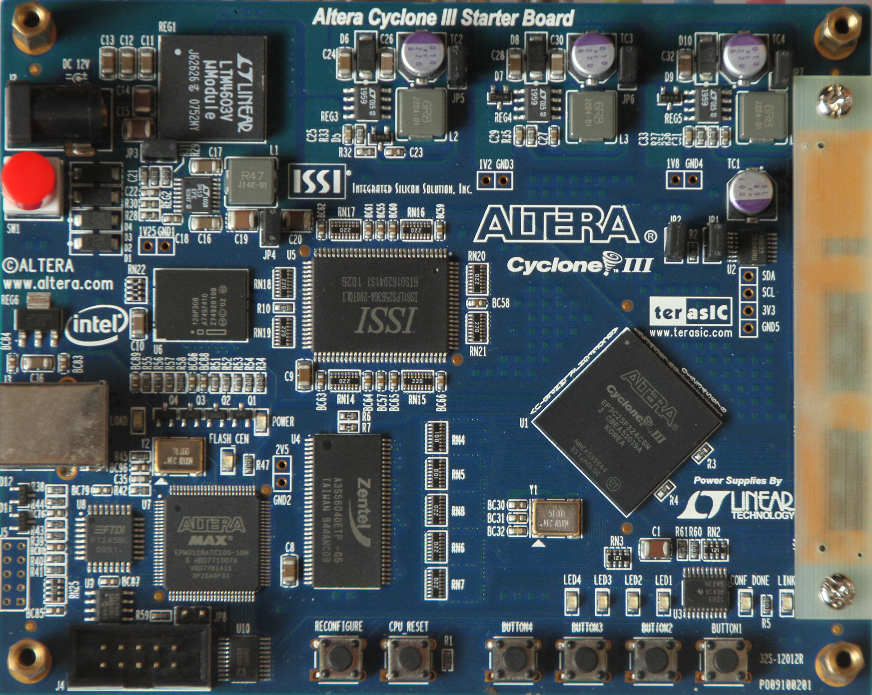
\includegraphics[width=\textwidth]{./figuras/NEEK/Trasera.png}
\caption{Vista Trasera NEEK}
\label{fig:traseraneek}
\end{figure}

\begin{figure}[p]
\centering
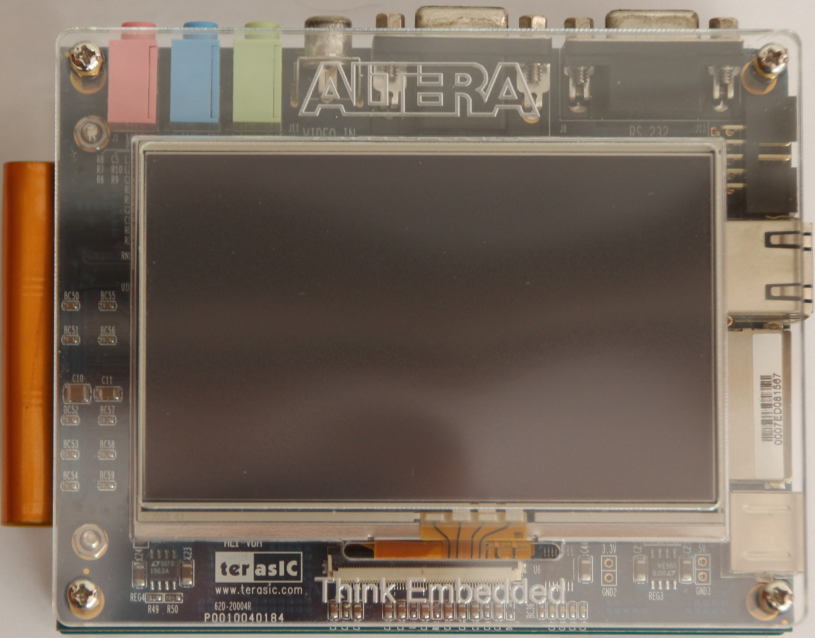
\includegraphics[width=\textwidth]{./figuras/NEEK/Delantera.png}
\caption{Vista Delantera NEEK}
\label{fig:delanteraneek}
\end{figure}

\paragraph{}
Si nos fijamos en la esquina inferior derecha de la parte trasera (figura~\ref{fig:traseraneek}), se puede ver un conjunto de botones y LEDs que se pueden ver con más detalle en la figura~\ref{fig:botonescontrol}.

\begin{figure}[p]
\centering
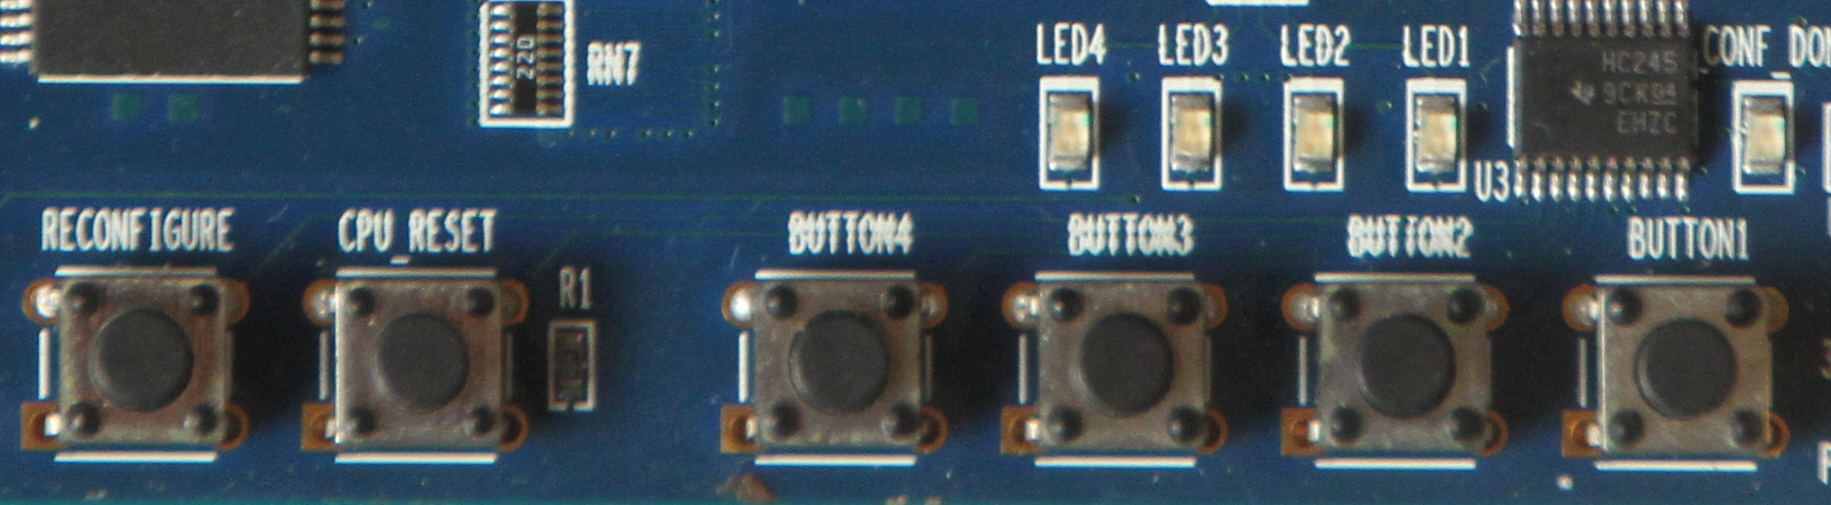
\includegraphics[width=0.95\textwidth]{./figuras/NEEK/BotonesSetup.png}
\caption{Botones de Control}
\label{fig:botonescontrol}
\end{figure}

\clearpage

\paragraph{}
Los botones etiquetados como \textit{Button n} controlaran las siguientes funciones del sistema:
\begin{itemize}
\item \textbf{Button 1:} Activar/desactivar contador de ciclos por frame.
\item \textbf{Button 2:} Selecciona entre los modos de \textit{Solo Vídeo} y \textit{Calculo del Sobel}.
\item \textbf{Button 3:} Activar/desactivar congelar un frame.
\item \textbf{Button 4:} Selecciona entre los modos \textit{Hardware} y \textit{Software} para calcular el Sobel. 
\end{itemize}

\paragraph{}
Además los botones etiquetados como:
\begin{itemize}
\item \textbf{Reconfigure:} Fuerza a que se descargue el archivo de configuración por defecto en la FPGA. 
\item \textbf{CPU\_Reset:} Reinicia el firmware.
\end{itemize}

\paragraph{}
Por otra parte el LED etiquetado como \textit{LED 4} se iluminara para indicar si el modo hardware esta activado. 

\paragraph{}
Si ahora nos fijamos en el lateral izquierdo de la figura~\ref{fig:traseraneek} podemos observar que hay un botón rojo y un conector USB. El botón rojo sirve para encender el \textit{NEEK}, él cual arrancará con una configuración FPGA por defecto. Para cargar la configuración del sistema de visión se utilizará la conexión USB. En la figura~\ref{fig:botonusb} se puede observar con mas detalle este área.

\paragraph{}
Por el tipo de licencia con el que se ha desarrollado el sistema, el único camino posible para cargar la configuración es mediante USB, teniendo que permanecer conectado y no siendo posible su carga desde la SD o cualquier tipo de memoria permanente.

\begin{figure}[p]
\centering
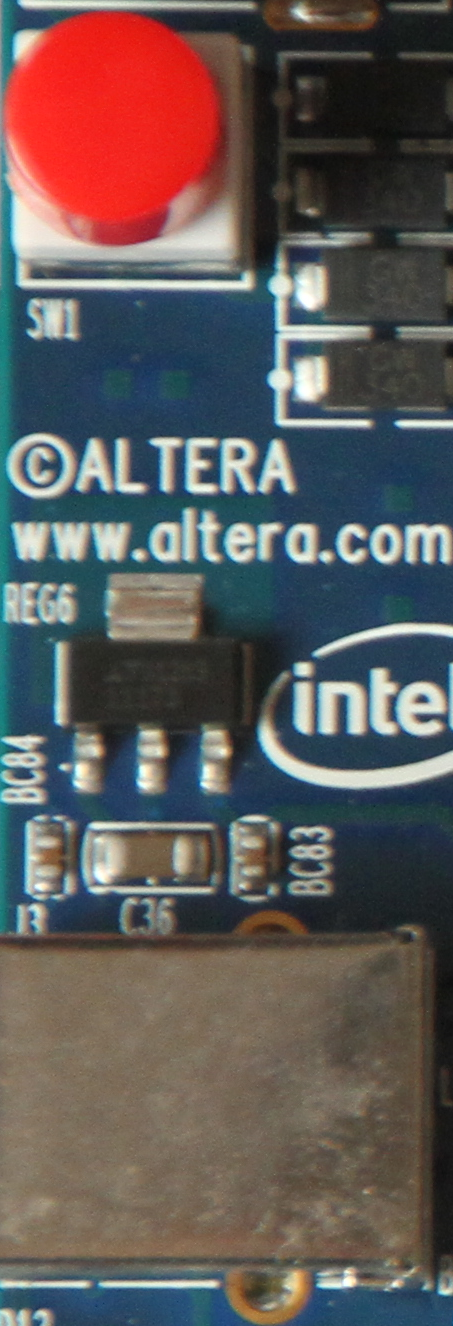
\includegraphics[width=0.2\textwidth]{./figuras/NEEK/BotonPowerUSB.png}
\caption{Botón Encendido y Conector USB}
\label{fig:botonusb}
\end{figure}

\paragraph{}
En la figura~\ref{fig:delanteraneek}, se puede ver el LCD donde se mostrara la imagen y la entrada de vídeo compuesto situada en la parte superior al lado de los conectores de audio. En la figura~\ref{fig:VIN} se puede apreciar mejor la entrada de vídeo.  

\begin{figure}[p]
\centering
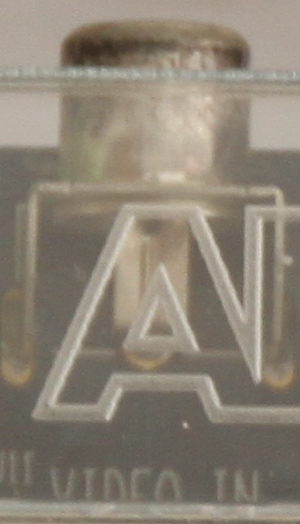
\includegraphics[width=0.20\textwidth]{./figuras/NEEK/VIN.png}
\caption{Entrada de Vídeo}
\label{fig:VIN}
\end{figure}

\clearpage
\section{Resultados}
\subsection*{}
\subsubsection*{}

\paragraph{}
En esta sección se mostrarán los resultados de los experimentos realizados. Para preparar los experimentos se tomaron varias muestras no consecutivas mediante el uso de la función congelar frame. La unidad utilizada en las medidas es el número de ciclos de CPU necesarios para dibujar un frame.


\paragraph{}
Se realizaron los siguientes experimentos:
\begin{itemize}
\item Comprobar los ciclos necesarios por frame de las funciones \textit{FrameWriter} y \textit{FrameReader} que generan un flujo de vídeo en color.
\item Comprobar los ciclos necesarios por frame para calcular el Sobel por Hardware.
\item Comprobar los ciclos necesarios por frame para calcular el Sobel por Software.
\end{itemize}

\paragraph{}
En la Tabla~\ref{tab:Muestras} se pueden observar las muestras obtenidas para cada prueba.

\begin{table}[hbtp]
\centering
\begin{tabular}{*{3}{c}}
Video   & Sobel Hardware & Sobel Sofware \\
\hline
3419643 &    9226067     &  3426726369   \\
3574272 &    9392345     &  3426370824   \\
3480150 &    9449637     &  3419864988   \\
3568071 &    9512463     &  3425147698   \\
3473887 &    9691520     &  3426242018   \\
3574626 &    9490562     &  3431587703   \\
3459205 &    9568320     &  3430750626   \\
3464364 &    9639976     &  3416688109   \\
3695883 &    9334261     &  3423139478   \\
3680720 &    9247614     &  3422926353   \\
\end{tabular}
\caption{Muestras}
\label{tab:Muestras}
\end{table}

\paragraph{}
En tabla~\ref{tab:resutadosc} se puede observar la media aritmética de cada experimento. Como se puede observar la version hardware del Sobel es unas 360 veces más rápida que la versión software.

\begin{table}[hbtp]
\centering
\begin{tabular}{l r}
Experimento            & Media Aritmética \\
\hline
Reproducción de Vídeo  &    3539082.1     \\
Sobel por Hardware     &    9455276.5     \\
Sobel por Software     &   3424944416.6   \\
\end{tabular}
\caption{Media de Ciclos por Frame}
\label{tab:resutadosc}
\end{table}

\paragraph{}
Sabiendo que la frecuencia del sistema es de unos 150Mhz, se puede determinar el numero de frames por segundo que se generan. En la tabla~\ref{tab:resutadosf} se puede comprobar estos valores.

\begin{table}[hbtp]
\centering
\begin{tabular}{l r}
Experimento            & FPS \\
\hline
Reproducción de Vídeo  & 42.38 \\
Sobel por Hardware     & 16.26 \\
Sobel por Software     & 0.044 \\
\end{tabular}
\caption{Media de Frames por Segundo}
\label{tab:resutadosf}
\end{table}

\paragraph{}
Como se puede comprobar la reproducción de vídeo es capaz de soportar el formato PAL sin perder ningún frame. Por otra parte el Sobel calculado por hardware mantiene un Framerate de aproximadamente 16 FPS frente a los 25 totales del formato PAL, lo que permite ver con bastante fluidez un vídeo. Finalmente la version software necesita casi 23 segundos para generar un solo frame, lo que la hace altamente ineficiente.

\appendix
\cleardoublepage % \clearpage 
\pagestyle{empty}
\appendixpage
\noappendicestocpagenum
\addappheadtotoc

\chapter{''Código Fuente Verilog''}

\subsubsection{Rawapro}
\raggedbottom
\lstinputlisting[caption=RawaPro.v,label=lst:RawaProv]{./SISSources/V/RawaPro.v}
\flushbottom
\clearpage

\subsubsection{Sobel Instruction Set}
\raggedbottom
\lstinputlisting[caption=SIS.v,label=lst:SISv]{./SISSources/V/SIS.v}
\flushbottom
\clearpage

\subsubsection{RAM Write}
\raggedbottom
\lstinputlisting[caption=ram\_w.v,label=lst:ramwv]{./SISSources/V/ram_w.v}
\flushbottom
\clearpage

\subsubsection{RAM Read}
\raggedbottom
\lstinputlisting[caption=ram\_r.v,label=lst:ramrv]{./SISSources/V/ram_r.v}
\flushbottom
\clearpage

\subsubsection{FrameWriter}
\raggedbottom
\lstinputlisting[caption=FrameWriter.v,label=lst:FrameWriterv]{./SISSources/V/FrameWriter.v}
\flushbottom
\clearpage

\subsubsection{AGrises}
\raggedbottom
\lstinputlisting[caption=AGrises.v,label=lst:AGrisesv]{./SISSources/V/AGrises.v}
\flushbottom
\clearpage

\subsubsection{Sobel}
\raggedbottom
\lstinputlisting[caption=Sobel.v,label=lst:Sobelv]{./SISSources/V/Sobel.v}
\flushbottom
\clearpage

\subsubsection{Sobel Cache}
\raggedbottom
\lstinputlisting[caption=Sobel\_cache.v,label=lst:Sobelcachev]{./SISSources/V/Sobel_cache.v}
\flushbottom
\clearpage

\chapter{''Código Fuente C''}
\lstset{
language=c
}

\subsubsection{Programa Principal}
\raggedbottom
\lstinputlisting[caption=main.c,label=lst:mainc]{./SISSources/C/main.c}
\flushbottom
\clearpage

\subsubsection{Keyhandler}
\raggedbottom
\lstinputlisting[caption=keyhandler.h,label=lst:keyhandlerh]{./SISSources/C/keyhandler.h}
\flushbottom
\clearpage

\raggedbottom
\lstinputlisting[caption=keyhandler.c,label=lst:keyhandlerc]{./SISSources/C/keyhandler.c}
\flushbottom
\clearpage

\subsubsection{Sobel Function Set}
\raggedbottom
\lstinputlisting[caption=sfs.h,label=lst:sfsh]{./SISSources/C/sfs.h}
\flushbottom
\clearpage

\raggedbottom
\lstinputlisting[caption=sfs.c,label=lst:sfsc]{./SISSources/C/sfs.c}
\flushbottom
\clearpage

\subsubsection{System Alias}
\raggedbottom
\lstinputlisting[caption=system\_alias.h,label=lst:systemaliash]{./SISSources/C/system_alias.h}
\flushbottom
\clearpage

\subsubsection{ALT TPO LCD}
\raggedbottom
\lstinputlisting[caption=alt\_tpo\_lcd.h,label=lst:alttpolcdh]{./SISSources/C/alt_tpo_lcd.h}
\flushbottom
\clearpage

\subsubsection{TV Decoder}
\raggedbottom
\lstinputlisting[caption=tvdecoder\_ctrl.h,label=lst:tvdecoderctrlh]{./SISSources/C/tvdecoder_ctrl.h}
\flushbottom
\clearpage

\raggedbottom
\lstinputlisting[caption=i2c.h,label=lst:i2ch]{./SISSources/C/i2c.h}
\flushbottom
\clearpage

\subsubsection{Simple Graphics}

\raggedbottom
\lstinputlisting[caption=simple\_graphics.h,label=lst:simplegraphicsh]{./SISSources/C/simple_graphics.h}
\flushbottom
\clearpage

\raggedbottom
\lstinputlisting[caption=alt\_video\_display.h,label=lst:altvideodisplayh]{./SISSources/C/alt_video_display.h}
\flushbottom
\clearpage

\raggedbottom
\lstinputlisting[caption=fonts.h,label=lst:fontsh]{./SISSources/C/fonts.h}
\flushbottom
\clearpage

\subsubsection{FrameReader}
\raggedbottom
\lstinputlisting[caption=vip\_wrapper\_for\_c\_func.h,label=lst:vipwrapperforcfunc]{./SISSources/C/vip_wrapper_for_c_func.h}
\flushbottom
\clearpage

\backmatter

\bibliographystyle{abbrvnat}
\bibliography{biblio}

\end{document}
